\documentclass[fleqn, a4paper, 12pt]{article}
\usepackage{amsmath, amssymb, amsthm, esdiff}
\usepackage[table]{xcolor}
\usepackage{commath}
\usepackage{gensymb}
\usepackage{hyperref}
\usepackage{tikz, pgfplots}
\usetikzlibrary{calc}
\usepackage{datetime}
\usepackage{setspace}
\usepackage{ulem}

\usepackage{enumerate, enumitem}

\setcounter{secnumdepth}{4}

\newcommand\numberthis{\addtocounter{equation}{1}\tag{\theequation}}

\theoremstyle{definition}
\newtheorem{example}{Example}
\newtheorem{definition}{Definition}

\theoremstyle{theorem}
\newtheorem{theorem}{Theorem}
\newtheorem{corollary}{Corollary}

\theoremstyle{remark}
\newtheorem{remark}{Remark}
\newtheorem{case}{Case}

\newenvironment{solution}
{\begin{proof}[Solution]\let\qed\relax}
	{\end{proof}}

\makeatletter
\@addtoreset{corollary}{theorem} %resets corollary numbers after a theorem
\makeatother

%opening
\title{Lecture 13}
\author{Aakash Jog}
\date{\formatdate{4}{12}{2014}}

\begin{document}
	
\maketitle
%\setlength{\mathindent}{0pt}

\tableofcontents

\newpage

\section{Definite Integrals}

\subsection{Definition}

\begin{example}
	Calculate an area $S$ which is situated between $y = f(x) = x^2$ and the $x$-axis on $[0, b]$.
\end{example}

\begin{solution}
	Divide $[0, b]$ on $n$ sub-intervals.\\
	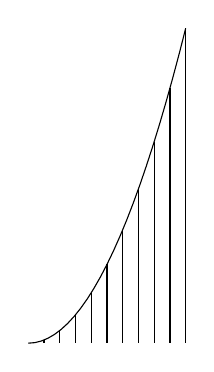
\begin{tikzpicture}
		\draw plot [domain = 0:2] (\x, {pow(\x,2)});
			
		\foreach \x in {0.2, 0.4, ..., 2}
		{
			\draw (\x, {pow(\x,2)}) -- (\x,0);
		}
	\end{tikzpicture}\\
	Therefore, for $i = 1, \dots, n$,
	\begin{align*}
		\Delta x_i &= x _i - x_{i - 1} \\
		&= \dfrac{b}{n}
	\end{align*}
	Therefore, for $i = 0, \dots, n$,
	\begin{align*}
		x_i = \dfrac{i b}{n}
	\end{align*}
	Let $S_n$ be the sum of areas of rectangles below the function.\\
	Let $\overline{S_n}$ be the sum of areas of rectangles above the function.
	
	\begin{align*}
		\sum_{k = 1}^{n} k^2 &= \dfrac{(n)(n + 1)(2n + 1)}{6}\\
		\therefore \underline{S_n} &= \sum_{i = 1}^{n} f(x_{i - 1}) \Delta x_i\\
		&= \sum_{i = 1}^{n} x_{i - 1}^2 \Delta x_0\\
		&= \sum_{i = 1}^{n} \dfrac{(i - 1)^2 b^2}{n^2} \cdot \dfrac{b}{n}\\
		&= \dfrac{b^3}{n^3} \cdot \dfrac{(n)(n - 1)(2n + 1)}{6}\\
		\therefore \overline{S_n} &= \sum_{i = 1}^{n} f(x_i) \Delta x_i\\
		&= \sum_{i = 1}^{n} x_i^2 \Delta x_0\\
		&= \sum_{i = 1}^{n} \dfrac{i^2 b^2}{n^2} \cdot \dfrac{b}{n}\\
		&= \dfrac{b^3}{n^3} \cdot \dfrac{(n)(n - 1)(2n + 1)}{6}
	\end{align*}
	$\forall n \in \mathbb{N}$,
	\begin{align*}
		S_n \leq S \leq \overline{S_n}\\
	\end{align*}
	Also,
	\begin{align*}
		\lim\limits_{n \to \infty} \overline{S_n} = \dfrac{b^3}{3} = \lim\limits_{n \to \infty} \underline{S_n}
	\end{align*}
	Therefore, by the Sandwich Rule,
	\begin{align*}
		\lim\limits_{n \to \infty} S = S = \dfrac{b^3}{3}
	\end{align*}
\end{solution}

\begin{definition}[Riemann integral sum]
	Let $f(x)$ be defined on the closed interval $[a, b]$. Let $n \in \mathbb{N}$ and $T$ be a partition of $[a, b]$ on $n$ sub-intervals, i.e.
	\begin{equation*}
		a = x_0 < x_1 < \dots < x_i < \dots < x_{n-1} < x_n = b
	\end{equation*}
	Let $\Delta x_i = x_i - x_{i - 1}$.\\
	$\Delta T = \max\{\Delta x_i\}$ is called the \emph{norm of the partition $T$}.\\
	For $c_i \in [x_{i-1, x_i}]$, $\sum_{i = 1}^{n} f(c_i) \Delta x_i$ is called the \emph{Riemann integral sum} corresponding to $T$.
\end{definition}

\begin{definition}[Definite integral]
	A function $f(x)$ is called integrable by Riemann over $[a, b]$ if $\exists I = \lim\limits_{\Delta T \to 0} \sum_{i = 1}^{n} f(c_i) \Delta x_i$ and the limit does not depend on the choice of $T$ and $c_i$. This limit is denoted by 
	\begin{equation*}
		I = \int\limits_{a}^{b} f(x) \dif x
	\end{equation*}
	and is called the \emph{definite integral} or the \emph{Riemann integral} of $f(x)$ over $[a, b]$.
\end{definition}

\subsection{Integrability}

\begin{theorem}
	If $f(x)$ is not bounded on $[a, b]$, then $f(x)$ is not integrable by Riemann over $[a, b]$.
\end{theorem}

\begin{corollary}
	If $f(x)$ is integrable over $[a, b]$ then $f(x)$ is bounded on $[a, b]$.
\end{corollary}

\begin{definition}
	A function $f(x)$ which is defined and bounded on $[a, b]$ is called \emph{piecewise continuous} if it has at most a finite number of discontinuous point and all of these are removable discontinuity points or discontinuous points of the first kind.
\end{definition}

\begin{theorem}
	If $f(x)$ is piecewise continuous on $[a, b]$, then $f(x)$ is Riemann integrable over $[a, b]$.
\end{theorem}

\begin{theorem}
	If $f(x)$ is bounded and monotonic on $[a, b]$, then $f(x)$ is Riemann integrable over $[a, b]$.
\end{theorem}

\subsection{Properties}
If all following integrals exist, and $a, b, c \in \mathbb{R}$
\begin{align*}
	\int\limits_{a}^{a} f(x) \dif x &= 0\\
	\int\limits_{a}^{b} f(x) \dif x &= - \int\limits_{b}^{a} f(x) \dif x\\
	\int\limits_{a}^{b} x \dif x &= c (b - a)\\
	\int\limits_{a}^{b} (f(x) \pm g(x)) \dif x &= \int\limits_{a}^{b} f(x) \dif x \pm \int\limits_{a}^{b} g(x) \dif x\\
	\int\limits_{a}^{b} c f(x) \dif x &= c \int\limits_{a}^{b} f(x) \dif x\\
	\int\limits_{a}^{b} f(x) \dif x &= \int\limits_{a}^{c} f(x) \dif x + \int\limits_{b}^{c} f(x) \dif x\\
	f(x)  \geq 0 \forall x \in [a, b] &\implies \int\limits_{a}^{b} f(x) \dif x \geq 0\\
	f(x)  \geq g(x) \forall x \in [a, b] &\implies \int\limits_{a}^{b} f(x) \dif x \geq \int\limits_{a}^{b} g(x) \dif x\\
	m \leq f(x) \leq M \forall x \in [a, b] &\implies m (b - a) \leq \int\limits_{a}^{b} f(x) \dif x \leq M (b - a)\\
	\left| \int\limits_{a}^{b} f(x) \dif x \right| &\leq \int\limits_{a}^{b} \left| f(x) \right| \dif x
\end{align*}

\begin{theorem}[Integral Intermediate Value Theorem] \label{Integral Intermediate Value Theorem}
	If $f(x)$ is continuous on $[a, b]$, then $\exists c \in [a, b]$ s.t. 
	\begin{equation*}
		\int\limits_{a}^{b} f(x) \dif x = f(c) (b - a)
	\end{equation*}
\end{theorem}

\begin{theorem}[Fundamental Theorem of Calculus, Part 1]\label{Fundamental Theorem of Calculus, Part 1}
	Let $f(x)$ be continuous on $(a, b)$ and let $c \in (a, b)$. Then, the function $F(x) = \int\limits_{c}^{x} f(t) \dif t$ is an anti-derivative function of $f(x)$ on $(a, b)$, i.e.
	\begin{equation*}
		F'(x) = f(x) \quad ; \quad \forall x \in (a, b)
	\end{equation*}
\end{theorem}

\begin{proof}
	For any $x \in (a, b)$ and $x + \Delta x \in (a, b)$, 
	\begin{align*}
		F(x + \Delta x) - F(x) &= \int\limits_{c}^{x + \Delta x} f(t) \dif t - \int\limits_{c}^{x} f(t) \dif t\\
		&= \int\limits_{c}^{x} f(t) \dif t + \int\limits_{x}^{x + \Delta x} f(t) \dif t - \int\limits_{c}^{x} f(t) \dif t\\
		&= \int\limits_{x}^{x + \Delta x} f(t) \dif t
		\intertext{By \nameref{Integral Intermediate Value Theorem}, $\exists d \in [x, x + \Delta x]$} \\
		\therefore \int\limits_{x}^{x + \Delta x} f(t) \dif t &= f(d) \Delta x\\
		\therefore \dfrac{F(x + \Delta x) - F(x)}{\Delta x} &= f(d)\\
		\therefore F'(x) &= \lim\limits_{\Delta x \to 0} \dfrac{F(x + \Delta x) - F(x)}{\Delta x}\\
		&= \lim\limits_{\Delta x \to 0} f(d)\\
		&= f(x)
	\end{align*}
\end{proof}

\begin{theorem}[Fundamental Theorem of Calculus, Part 2]
	Let $f(x)$ be continuous on $[a, b]$ and let $G(x)$ be an arbitrary anti-derivative function of $f(x)$. Then,
	\begin{equation*}
		\int\limits_{a}^{b} f(x) \dif x = G(b) - G(a)
	\end{equation*}
\end{theorem}

\begin{proof}
	Let $d$ be an arbitrary point in $(a, b)$.\\
	By \nameref{Fundamental Theorem of Calculus, Part 1}, 
	\begin{equation*}
		F(x) = \int\limits_{d}^{x} f(t) \dif t
	\end{equation*}
	is an anti-derivative function of $f(x)$ on $[a, b]$.\\
	Therefore, for any other anti-derivative function $G(x) = F(x) + c$,
	\begin{align*}
		G(b) - G(a) &= (F(b) + c) 0 (F(a) + c)\\
		&= F(b) - F(a)\\
		&= \int\limits_{d}^{b} f(t) \dif t - \int\limits_{d}^{a} f(t) \dif t\\
		&= \int\limits_{d}^{a} f(t) \dif t + \int\limits_{a}^{b} f(t) \dif t - \int\limits_{d}^{a} f(t) \dif t\\
		&= \int\limits_{a}^{b} f(t) \dif t
	\end{align*}
\end{proof}

\end{document}
